\documentclass[10pt,twocolumn,letterpaper]{article}
\usepackage[margin=0.65in,columnsep=0.26in]{geometry}
\usepackage[OT1]{fontenc}
\usepackage{amsmath,amssymb,graphicx,booktabs,array}
\usepackage[font=small,labelfont=bf]{caption}
\usepackage{xcolor}
\usepackage[colorlinks=true,linkcolor=teal,citecolor=teal,urlcolor=teal]{hyperref}
\usepackage{microtype}
\newcommand{\R}{\mathbb{R}}
\newcommand{\norm}[1]{\left\lVert#1\right\rVert}
\newcommand{\src}{\mathrm{s}}
\newcommand{\tgt}{\mathrm{t}}
\newcommand{\bd}{\mathcal{B}}
\newcommand{\dyn}{\mathcal{D}}
\newcommand{\cat}{\mathcal{C}}
\newcommand{\free}{\mathcal{F}}
\newcommand{\one}{\mathbf{1}}
\DeclareMathOperator*{\argmin}{arg\,min}
\newcommand{\ResponseRows}{%
Jacket / macro & 8,885 & 3 & 2.216912 & 2.216912 & 2.150180 & 2.094106 & 5.539\% \\
Jacket / terminal & 1,514 & 4 & 4.943749 & 4.943749 & 4.615955 & 2.435535 & 50.735\% \\
Skirt outfit / macro & 4,009 & 4 & 3.828860 & 3.455767 & 3.350889 & 3.341212 & 12.736\% \\
Skirt outfit / terminal & 986 & 8 & 7.373308 & 7.373308 & 7.373308 & 7.372434 & 0.012\% \\
}

\newcommand{\SemanticRows}{%
Jacket & Native & 28 & 9.68e-01 & 9.38e-01 & 0 \\
Jacket & Native + B/D & 28 & 9.59e-01 & 0.00e+00 & 0 \\
Jacket & SBCST init. & 0 & 5.03e-08 & 0.00e+00 & 0 \\
Jacket & SBCST final & 0 & 4.57e-08 & 0.00e+00 & 0 \\
Skirt outfit & Native & 2,175 & 1.00e+00 & 1.00e+00 & 1,855 \\
Skirt outfit & Native + B/D & 320 & 4.70e-01 & 0.00e+00 & 0 \\
Skirt outfit & SBCST init. & 0 & 4.47e-08 & 0.00e+00 & 0 \\
Skirt outfit & SBCST final & 0 & 4.28e-08 & 0.00e+00 & 0 \\
}

\setlength{\emergencystretch}{1.5em}
\setlength{\textfloatsep}{12pt plus 2pt minus 2pt}
\setlength{\floatsep}{10pt plus 2pt minus 2pt}
\setlength{\abovedisplayskip}{6pt plus 2pt minus 2pt}
\setlength{\belowdisplayskip}{6pt plus 2pt minus 2pt}
\makeatletter
\renewcommand\section{\@startsection{section}{1}{\z@}{-2.0ex plus -.5ex minus -.2ex}{.9ex plus .2ex}{\normalfont\large\bfseries\raggedright}}
\renewcommand\subsection{\@startsection{subsection}{2}{\z@}{-1.8ex plus -.5ex minus -.2ex}{.7ex plus .2ex}{\normalfont\normalsize\bfseries\raggedright}}
\makeatother
\title{\vspace{-1.4em}\textbf{Semantic Budget-Constrained Skinning Transfer\\for Garment Retargeting}}
\author{tomTomIEE\\\small Independent Research\\\small\href{https://github.com/tomTom1010-IEE/KK_Modder-BatchTool}{KK Modder BatchTool}}
\date{\small Technical manuscript \;\textbullet\; September 2026}
\hypersetup{pdftitle={Semantic Budget-Constrained Skinning Transfer for Garment Retargeting},pdfauthor={tomTomIEE},pdfsubject={Semantic influence conservation and constrained garment skinning transfer},pdfkeywords={skinning, garment retargeting, semantic budgets, quadratic programming}}
\begin{document}
\raggedbottom
\maketitle

\begin{abstract}
Retargeting a skinned garment to a different character requires preserving an authored allocation of body and secondary-motion influence while adapting to new geometry and skeletal structure. Purely spatial weight transfer can cross semantic boundaries in layered clothing, introduce body influence into freely moving panels, and generate discontinuities on extended footwear. We present \emph{Semantic Budget-Constrained Skinning Transfer} (SBCST), a framework that separates the amount of influence assigned to a semantic category from its distribution among target bones. Per-vertex source budgets define a feasible set; native surface samples and reviewed semantic mappings initialize distributions within that set. Fixed-transform quadratic fitting then adapts body response using paired garment rest geometry, followed by optional local terminal refinement. A complementary footwear formulation regularizes spatial influence fields and fits pose-dependent separation. Explicit contact-review masks support scoped validation in the presence of authored intersections. In two local garment studies, initialization eliminates all measured wrong-category vertices (28 and 2,175), while preserving budgets to approximately $5\times10^{-8}$ after writeback. Final held-out response reductions relative to native transfer range from 0.012\% to 50.735\% across four evaluation scopes. A shoe study reduces held-out separation error by 4.990\%. These results establish a working constrained transfer pipeline and initial cross-rig applicability, with broader generalization and continuous collision guarantees left open.
\end{abstract}
\noindent\textbf{Keywords:} skinning transfer, garment retargeting, semantic influence budgets, constrained optimization, secondary motion.

\section{Introduction}
A garment's skinning weights encode design decisions that are not recoverable from proximity alone. An open panel can be almost entirely controlled by clothing bones, with a narrow transition into body motion near its attachment. A comparatively rigid accessory can instead retain a low, spatially uniform contribution from an arm bone. A collar and a sleeve may be close in space while belonging to different deformation domains. Transferring weights from the nearest body surface treats these situations similarly, even though their intended responses differ.

Changing character proportions compounds the problem. The fitted garment can have different limb lengths, local offsets, and surface shape from its original version. The target body may contain more deformation segments or helper bones, and its mesh need not correspond to the source body. Copying bone names cannot reproduce those distributions; comparing posed vertices in absolute world coordinates penalizes the intentional change of shape itself.

We formulate transfer as the preservation of \emph{semantic influence budgets}. Each source vertex allocates a normalized amount of influence to broad body categories and to retained clothing bones. This allocation remains fixed, while weights within a target body category are allowed to change. The central distinction is between \emph{which category may act} and \emph{how its allowed share should be distributed}. Geometry supplies evidence for the latter, not permission to override the former.

Our implementation uses six categories: torso (including head and neck), the four individual limbs, and retained dynamic influence. The formulation admits other partitions; six is an implementation choice, not a requirement of the mathematics. Selected finger weights are reserved inside their limb budgets rather than creating additional categories. Clothing-bone weights remain fixed individually, so optimization cannot consume a free panel's secondary-motion allocation to improve a body-response metric.

SBCST combines this constraint with two fitting objectives. For ordinary garments, we transport source motion through paired original/fitted rest geometry and anatomical frames, then optimize target body weights. For extended flat shoes, we instead preserve spatial association to the target foot and optionally refine separation over poses. Both share fixed budgets, admissible target-bone support, and independent validation.

Our contributions are (1) a practical decomposition of garment transfer into conserved semantic budgets and adaptable within-category distributions; (2) a fixed-transform fitting pipeline with proportion-aware motion transport and bounded terminal refinement; and (3) an inspectable implementation with spatial footwear fitting, explicit review boundaries, and same-input quantitative comparisons. We present a technical method and local evidence, rather than claiming a universally automatic retargeting solution or a new skinning decomposition algorithm.

\begin{figure*}[t]
\centering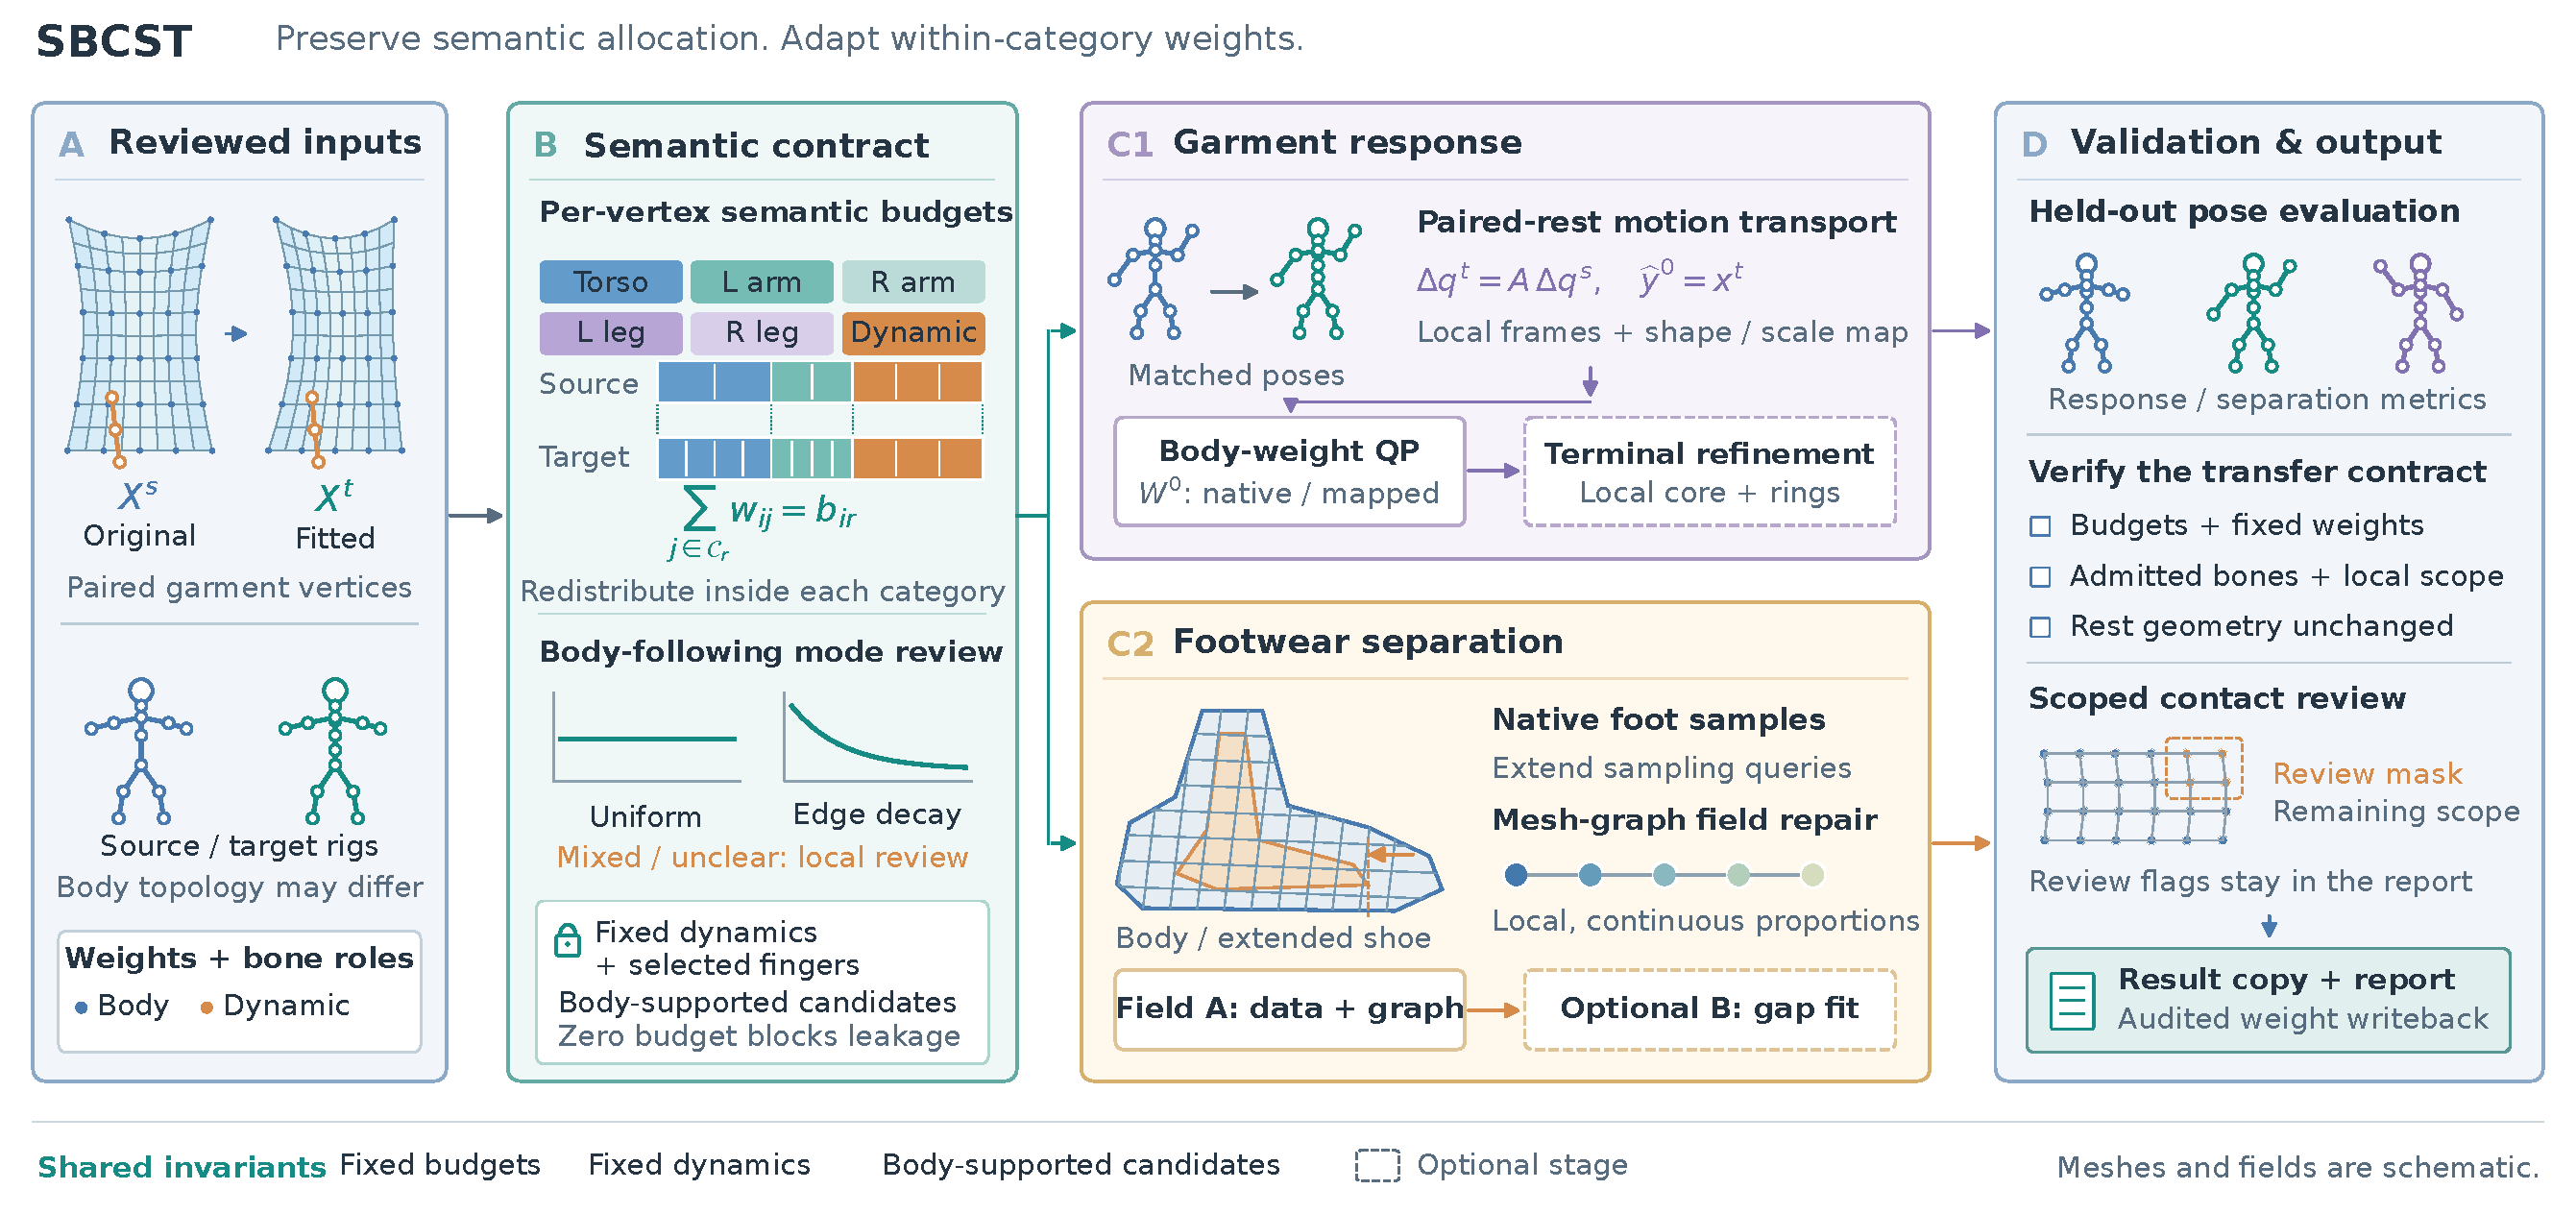
\includegraphics[width=\textwidth]{figures/pipeline.pdf}
\caption{SBCST architecture. (A) Paired garment geometry and reviewed rig inputs. (B) Per-vertex semantic budgets preserve allocation while allowing redistribution among target bones. (C1) Garment-response fitting transports source motion; (C2) footwear fitting preserves target-body spatial association. (D) Independent validation checks invariants, held-out response, and explicitly reviewed contact scopes. Dashed stages are optional; meshes, weights, and feature curves are schematic.}
\label{fig:pipeline}
\end{figure*}

\section{Related Work and Scope}
\paragraph{Skinning decomposition.}
Smooth Skinning Decomposition with Rigid Bones (SSDR) estimates rigid transformations and a sparse convex weight map from example deformations through alternating optimization~\cite{ssdr}. SBCST addresses a different setting: both rigs and their sampled transformations are given. We adapt existing weights under semantic equality constraints, without recovering a skeleton, alternating over bone transformations, or enforcing SSDR's bone-count sparsity model. The shared least-squares structure should not be interpreted as equivalent objectives or comparable benchmark results.

\paragraph{Smooth influence fields.}
Bounded biharmonic weights construct smooth, bounded influence fields through a variational formulation~\cite{bbw}. This motivates the value of geometry-aware regularity, but our footwear solver operates on a surface adjacency graph initialized by native surface transfer. It does not solve a volumetric biharmonic problem. Regularity and semantic allocation are complementary: smoothing an unconstrained field cannot determine whether a nearby sleeve bone is appropriate for a collar.

\paragraph{Surface transfer and quadratic fitting.}
The implementation uses Blender's native nearest-face-interpolated vertex-group transfer as its sampling primitive~\cite{blender}. We retain it as a useful initial estimator, then restrict its authority through semantic budgets. With fixed pose matrices and references, our garment objective yields sparse convex quadratic subproblems solved with OSQP~\cite{osqp}. Contacts are updated sequentially; convexity of an individual subproblem does not imply global collision avoidance.

\paragraph{What is outside the problem.}
Static fitting and clothing-bone grafting precede weight transfer. SBCST assumes these inputs have been reviewed, and does not change garment vertices during optimization. It does not identify secondary-motion inertia, damping, or runtime collision parameters. Retaining clothing-bone influence preserves an attachment mechanism, not an entire physical trajectory. Similarly, matching a discrete pose set does not establish correctness for arbitrary continuous animation or body-shape edits.

\section{Problem Formulation}
\label{sec:formulation}
Let $X^\src,X^\tgt\in\R^{n\times3}$ be original and fitted garment rest positions with corresponding vertex indices and connectivity. Source and target \emph{body} meshes may have different topology. Let $W^\src$ be effective nonnegative source weights and $W\in\R^{n\times m}$ the target weights. All positions and transforms are expressed in a common world-space convention; mesh and armature object transforms are included in the evaluated skinning matrices.

For pose $p$, let $T_j^p$ be the fixed homogeneous target skinning transform, including the inverse bind transform. Define $a_{ij}^p=\pi(T_j^p\bar x_i^\tgt)$, where $\pi$ retains the spatial coordinates and $\bar x$ appends a homogeneous one. Linear blend skinning (LBS) is
\begin{equation}
 y_i^p(W)=\sum_{j=1}^{m}w_{ij}a_{ij}^p,
 \qquad w_{ij}\geq0,\quad\sum_jw_{ij}=1.
 \label{eq:lbs}
\end{equation}
The source response is evaluated using all effective source deformation influences, including supported helper bones. A bone used as a pose control or anatomical reference is not necessarily a valid recipient of target weights.

\subsection{Semantic budgets and fixed contributions}
Every source influence receives a reviewed role: body, retained dynamic, explicitly discarded, or non-deforming. The classification uses actual deformation participation and rig semantics. A bone outside a standard humanoid list is not automatically a clothing physics bone.

Let $\bd_\src$ and $\dyn_\src$ be the valid body and retained dynamic sets. For $s_i>0$, define
\begin{align}
 s_i&=\sum_{j\in\bd_\src\cup\dyn_\src}w^\src_{ij},
 &\widetilde w^\src_{ij}&=w^\src_{ij}/s_i,\label{eq:normalize}\\
 b_{ir}&=\sum_{j\in\cat_r^\src}\widetilde w^\src_{ij},
 &\sum_{r=1}^{K}b_{ir}&=1.\label{eq:budget}
\end{align}
The sets $\cat_r^\src$ partition the valid influences. Vertices without valid mass are unresolved inputs, not implicitly pure-dynamic vertices. For corresponding target categories $\cat_r^\tgt$, transfer satisfies
\begin{equation}
 \sum_{j\in\cat_r^\tgt}w_{ij}=b_{ir}\quad\forall i,r.
 \label{eq:conserve}
\end{equation}
With the six-category partition, Equation~\eqref{eq:conserve} refines conservation of the total body/dynamic split. The latter alone would allow all body mass to migrate from torso to arm.

Retained dynamic weights are fixed after normalization and approved bone correspondence. Enabled finger contributions are also mapped and reserved individually. Denote all such fixed contributions by $f_{ij}$, their index set by $\mathcal{P}_i$, and the remaining category mass by
\begin{equation}
 \beta_{ir}=b_{ir}-\sum_{j\in\cat_r^\tgt\cap\mathcal{P}_i}f_{ij}.
 \label{eq:residualbudget}
\end{equation}
We reject negative residual mass or positive residual mass without admissible recipients. Disabled source fingers are explicitly redistributed to same-side non-finger body bones; they are not deleted and followed by unrestricted renormalization. An entire forefoot control is not an individual finger and remains part of its leg category.

\subsection{Admissible support}
Let $u_{vj}$ be target-body weights. A target body bone is globally eligible only if it has positive support on that body. Per-vertex candidate sets further restrict this pool:
\begin{equation}
 \free_i\subseteq\{j\in\bd_\tgt:\exists v,\ u_{vj}>0\}.
 \label{eq:support}
\end{equation}
Weights outside admitted or fixed support are zero. Eligibility is necessary but not sufficient. Same-side semantics, reviewed mappings, local surface evidence, and refinement scope restrict the actual recipients. Dynamic bones are admitted separately. This avoids assigning garment weights to control-only helpers or distant, merely available body bones.

\paragraph{Immediate consequence.}
If $b_{ir}=0$, nonnegativity and Equation~\eqref{eq:conserve} imply $w_{ij}=0$ for every $j\in\cat_r^\tgt$. Thus forbidden-category influence is excluded by construction, irrespective of spatial proximity. This is an allocation guarantee conditional on correct source semantics; it is not a statement about collision or perceptual quality.

\section{Feature-Aware Initialization}
\label{sec:init}
\subsection{Following patterns in dynamic regions}
We identify a region from the actual influence of a reviewed clothing-bone root and its descendants, with optional explicit vertex masks. A root is a convenient selection handle; its geometric vicinity is not the region definition. Overlapping or semantically ambiguous regions require resolution before automatic processing.

For body share $h_i=\sum_{j\in\bd_\src}\widetilde w^\src_{ij}$, define the conditional body distribution $q_{ij}=\widetilde w^\src_{ij}/h_i$ when $h_i>0$. Uniform following requires stability of \emph{both} $h_i$ and $q_i$: a constant total with changing bone identity is not a uniform mode. The implementation measures range, relative range, variance, and total-variation distance to a component mean,
\begin{equation}
 v_i=\tfrac12\sum_{j\in\bd_\src}|q_{ij}-\overline q_j|.
 \label{eq:tv}
\end{equation}
The current conservative rule accepts uniform components when the body-share range is at most 0.025, its ratio to the mean is at most 0.20, the 95th percentile of $v_i$ is at most 0.08, and its maximum is at most 0.18. These are engineering thresholds, not learned or statistically calibrated classifiers.

Attachment-edge decay is suggested only when shares decrease with graph distance from an adjacent body-dominated boundary. The implementation checks sufficient range, a low free-end share, at least four distance layers, reverse-edge frequency, and a decreasing isotonic fit. Its fit score is
\begin{equation}
 R^2_{\mathrm{decay}}=1-
 \frac{\sum_i(h_i-\widehat h(d_i))^2}{\sum_i(h_i-\overline h)^2},
 \label{eq:decay}
\end{equation}
where $d_i$ is topological boundary distance. The current minimum is 0.65, with additional checks on local jumps and total decay. Separate connected components must agree or be reviewed separately. Pure-dynamic components retain zero body mass and do not vote on a body-following label.

These statistics produce one of three suggestions: uniform, edge-gradient, or unresolved. A stable per-bone pedestal combined with a different varying component is explicitly unresolved. Treating the sum as one gradient would erase the stable component's identity. The reserved protected-component interface is not yet implemented; this case requires manual or Agent-assisted per-vertex analysis. Suggestions configure the estimator only after review; they do not override the source budgets.

\subsection{Combining native sampling and semantic mapping}
On temporary meshes, Blender's \texttt{POLYINTERP\_NEAREST} operator samples target-body vertex groups. After filtering finger recipients, let $p_{ij}$ be the conditional sampled distribution within category $r$, and let $m_{ij}$ be a normalized reviewed semantic mapping of residual source contributions. A confidence $\gamma_{ir}\in[0,1]$ initializes free entries as
\begin{equation}
 w^0_{ij}=\beta_{ir}\big[(1-\gamma_{ir})m_{ij}+\gamma_{ir}p_{ij}\big],
 \quad j\in\cat_r^\tgt\cap\free_i.
 \label{eq:init}
\end{equation}
Fixed contributions are then included unchanged. Uniform regions use $\gamma_{ir}=0$ to preserve their semantic following pattern. Reviewed gradient or ordinary body regions can use sampling. If the category accounts for less than the configured minimum sampled mass (0.05 by default), confidence falls back to zero. This prevents numerical amplification of negligible cross-region samples. If a reliable mapping is unavailable, the workflow stops rather than inventing support.

Both distributions in Equation~\eqref{eq:init} sum to one, so its free weights sum to $\beta_{ir}$ for every confidence. Therefore initialization is feasible before optimization. Explicit within-category policies, such as suppressing a localized shape-edit influence and reallocating its share to an enclosing body influence, preserve the same budget but remain application choices. They are not automatic consequences of the six-class model.

\section{Proportion-Aware Motion References}
\label{sec:transport}
Matching original and target posed vertices in world space would penalize intended changes in garment fit. Instead, SBCST transports only the source motion residual relative to anatomical frames, using paired garment geometry to estimate local changes of scale and shape.

For incident garment edges $e^\src_{ik}=x_k^\src-x_i^\src$ and $e^\tgt_{ik}=x_k^\tgt-x_i^\tgt$, define row matrices $E_i^\src,E_i^\tgt$ from these edges normalized by their source median length. Surface edge data are nearly rank two. We augment each matrix with a vertex-normal row; the target normal is scaled by the median local edge-length ratio. With a skeleton-derived prior $J_i^{\mathrm{prior}}$, fit
\begin{equation}
 J_i=\argmin_J\norm{E_i^\src J^T-E_i^\tgt}_F^2
             +\rho\norm{J-J_i^{\mathrm{prior}}}_F^2.
 \label{eq:jacobian}
\end{equation}
The implemented ridge is $\rho=0.05$. A local map is replaced by the explicit prior when input neighborhoods are degenerate, the determinant is nonpositive, or singular values fall outside $[0.2,5]$. These guards prevent a folded or severely altered neighborhood from defining an unstable motion scale. Fallback indices are reportable diagnostics.

Let $H_i^{\src,p}$ and $H_i^{\tgt,p}$ be rigid world-space anatomical frames with rotation blocks $R_i^{\src,p}$ and $R_i^{\tgt,p}$. The adapters construct corresponding macro actions rather than assuming identical bone-local Euler axes. Additional target spine segments can share a macro rotation through an explicit pose mapping. The complete evaluated source rig still determines the source garment deformation.

In local coordinates, define
\begin{align}
 q_i^{\src,p}&=\pi\big((H_i^{\src,p})^{-1}\bar y_i^{\src,p}\big),\\
 q_i^{\tgt,0}&=\pi\big((H_i^{\tgt,0})^{-1}\bar x_i^\tgt\big),\\
 A_i&=(R_i^{\tgt,0})^TJ_iR_i^{\src,0}.
\end{align}
The transported target is
\begin{equation}
 \widehat y_i^p=\pi\left(H_i^{\tgt,p}
 \begin{bmatrix}q_i^{\tgt,0}+A_i(q_i^{\src,p}-q_i^{\src,0})\\1\end{bmatrix}\right).
 \label{eq:reference}
\end{equation}
At rest the residual vanishes, hence $\widehat y_i^0=x_i^\tgt$ exactly. This preserves the fitted shape rather than pulling it back toward the original character. Rigid frame rotation and local scale are separated, avoiding double application of object scale or limb-length changes.

An anatomical anchor may use a helper bone's parent to avoid an artificial joint pivot. This affects the coordinate frame, not the source deformation calculation: the helper's own evaluated transform and weight remain in source LBS. Preserving this distinction is particularly relevant near wrists and twist-support chains.

\section{Constrained Response Optimization}
\label{sec:optimization}
\subsection{Objective and sparse quadratic program}
For training pose weights $\alpha_p\geq0$ normalized to sum to one, vertex weights $\omega_i\geq0$ normalized to mean one, and a positive length scale $\ell$, minimize
\begin{align}
 E(W)={}&\sum_{p,i}\frac{\alpha_p\omega_i}{\ell^2}
                   \norm{y_i^p(W)-\widehat y_i^p}^2\nonumber\\
       &+\lambda\norm{W-W^0}_F^2
        +\mu\norm{L(W-W^0)}_F^2.
 \label{eq:objective}
\end{align}
Here $L$ is an edge-incidence operator on the chosen garment graph. We smooth \emph{weight corrections}, not the source budget field. Smoothing budgets would blur attachment transitions and reintroduce body influence into intentionally free regions. The initialization prior stabilizes underdetermined responses and discourages unnecessary changes.

Eliminate fixed weights and vertices outside the selected scope. Stack the remaining weights into $z$, with initialization $z_0$. Equation~\eqref{eq:lbs} becomes affine in $z$; after pose, vertex, and length scaling, write its data residual as $Dz-r$. With the restricted correction graph $G$,
\begin{align}
 Q&=2(D^TD+\lambda I+\mu G^TG),\\
 c&=-2\big[D^Tr+(\lambda I+\mu G^TG)z_0\big].
\end{align}
The solve is
\begin{equation}
 \min_z\ \tfrac12z^TQz+c^Tz
 \quad\text{s.t.}\quad Sz=\beta,\quad l\leq z\leq u,
 \label{eq:qp}
\end{equation}
plus optional contact inequalities. The rows of $S$ encode residual category sums. Bounds include nonnegativity and per-vertex correction limits. Positive $\lambda$ makes the reduced Hessian positive definite; without it, correlated bone responses can leave multiple minimizers. With fixed references and linear constraints, each feasible subproblem is convex.

OSQP is warm-started from the feasible transferred weights. The implementation uses absolute and relative tolerances of $10^{-8}$, polishing, and a 20,000-iteration ceiling. Default coefficients are $\lambda=0.02$ and $\mu=0.01$; application configurations can override them. The length scale defaults to the fitted garment's bounding-box diagonal and can be specified for a local scope. These defaults describe the solver, not a claim that every archived experiment used an identical parameter set.

Tiny negative residuals are clamped and mass is repaired only within the same free category. Fixed contributions are never globally renormalized. Independent validation subsequently checks the written representation, since floating-point storage and numerical repair can differ from the mathematical solve.

\subsection{Contacts and scoped review}
For a posed contact sample, let $q$ and $n$ be the nearest body point and oriented normal at the current iterate. A local clearance constraint is
\begin{equation}
 n^T\big(y^p(z)-q\big)\geq\delta.
 \label{eq:contact}
\end{equation}
Vertex, edge-midpoint, and face-interior samples can be represented as barycentric combinations of garment vertices and remain affine in $z$. Updating correspondences between QP solves yields sequential contact subproblems. A trust bound limits each update. The nearest-face normal is an oriented contact proxy, not a watertight inside/outside oracle.

If a violating sample depends exclusively on frozen weights, the solver reports a fixed-contact conflict rather than changing conserved dynamics. Such a conflict can reflect authored geometry, an intentional cap, or an unsuitable fitted rest state. The correct response may be a geometry correction or an explicitly reviewed exception, not weight redistribution.

Let $\mathcal E$ denote a recorded contact-exemption mask and $\mathcal V$ the evaluation scope. Contact checks apply to $\mathcal V\setminus\mathcal E$, while budget and fixed-weight checks still apply throughout. Existing and newly introduced contact sets are distinguished:
\begin{equation}
 \mathcal C_{\mathrm{new}}=
 (\mathcal C_{\mathrm{after}}\setminus\mathcal C_{\mathrm{before}})
 \cap(\mathcal V\setminus\mathcal E).
 \label{eq:newcontact}
\end{equation}
This supports localized review without disabling validation globally. However, $\mathcal C_{\mathrm{new}}=\varnothing$ means no newly flagged vertices under the recorded test, not that all existing contacts vanished or penetration depth improved. An exception-reviewed result and a strict contact pass are distinct outcomes. Explicit masks make this distinction auditable and prevent a local limitation from being silently generalized to the entire garment.

\subsection{Terminal refinement}
Macro motions may provide insufficient information near a wrist or other endpoint. An optional second stage begins from the macro result, moves only reviewed endpoint controls from a neutral body pose, and restricts free weights to a selected core plus transition rings. The exterior remains fixed. For a scope-dependent limit $\Delta_i$,
\begin{equation}
 |w_{ij}-w^{\mathrm{macro}}_{ij}|\leq\Delta_i.
 \label{eq:terminal}
\end{equation}
Outside the refinement scope, $\Delta_i=0$. Same-side candidates and reserved fingers remain constrained. Local residual scaling prevents whole-body dimensions from dominating a small endpoint fit. This stage improves local response without repeating unrelated macro fitting; a region already well represented by its initial weights can change negligibly.

\section{Spatial Fitting for Extended Footwear}
\label{sec:shoe}
Shoes with a long toe box can depart substantially from the original garment-to-body spatial relation. A response-preserving objective is then not always the best design target. The footwear branch retains semantic allocation but estimates conditional body proportions from the target foot, extending supported influence along the forefoot direction where necessary.

\subsection{Sampling extension and graph repair}
Let $b_i$ be a shoe vertex's body share and $p_i$ its conditional distribution over admissible same-side foot-region bones. Write $w_{ij}=b_ip_{ij}$, with $p_i\geq0$ and $\one^Tp_i=1$. Vertices with $b_i=0$ are excluded from this body solve.

Given a reviewed forward direction $d$ and the forward extent $a$ of the weighted foot surface, the temporary sampling query is
\begin{equation}
 x_i'=x_i^\tgt-\max(0,d^Tx_i^\tgt-a)d.
 \label{eq:extension}
\end{equation}
Native surface transfer is performed on these queries; the actual shoe geometry does not move. This extends the supported field into a long toe box instead of amplifying unreliable remote samples. Unsupported regions elsewhere require review. High heels require pose-conditioned fitting and are outside the tested flat-shoe scope.

The field-only result $P_A$ regularizes native proportions $P^0$:
\begin{equation}
 E_A(P)=\sum_i c_i\norm{p_i-p_i^0}^2
       +\eta\sum_{(i,k)\in\mathcal G}\norm{p_i-p_k}^2,
 \label{eq:shoeA}
\end{equation}
subject to candidate support and the simplex constraints. Confidence decreases with separation and local disagreement. The graph follows same-side mesh edges within nonzero-body scope; nearby disconnected layers are not connected by spatial nearest neighbors. Candidate support starts from observed native weights and expands through bounded topology rings. Projected Jacobi updates regularize the field while preserving the simplex. This targets isolated transfer artifacts without assuming a rigid cluster or a globally uniform shoe weight.

\subsection{Pose-based separation refinement}
An optional result $P_B$ preserves the fitted offset from a target-body reference triangle. Fix rest barycentric coordinates for each vertex's reference point $a_i^0$ and transport them to $a_i^p$. For an orthonormal triangle frame $F_i^p$, define
\begin{align}
 o_i&=(F_i^0)^T(x_i^\tgt-a_i^0),\\
 g_i^p&=a_i^p+F_i^po_i.
\end{align}
The quadratic surrogate is
\begin{align}
 E_B(P)={}&\sum_{p,i}\alpha_pc_i'
 \norm{D_s(F_i^p)^T\big(y_i^p(P)-g_i^p\big)/\ell_i}^2\nonumber\\
 &+\lambda_B\norm{P-P_A}_F^2+\mu_B\norm{LP}_F^2,\label{eq:shoeB}\\
 D_s^TD_s={}&\operatorname{diag}(0.03,0.03,1).
\end{align}
The normal offset dominates, while weak tangential terms discourage sliding. Distant references receive lower confidence. Retained dynamics and body budgets stay fixed. A projected-gradient solver uses a conservative Hessian/graph bound and projects onto each masked simplex. Stopping is based on iterate change; we do not report it as a certified global optimality gap.

Equation~\eqref{eq:shoeB} fits a fixed-reference offset surrogate, not the exact nearest-surface distance. Independent evaluation re-queries posed body surfaces. Shoe contacts currently act as acceptance gates rather than active repair inequalities, and refinement cannot be assumed to repair pre-existing intersections.

\subsection{Pose sampling}
The standard training set contains ankle flexion at $\pm20^\circ$, mirrored side inclination at $\pm10^\circ$, forefoot flexion at $+18^\circ$ and $-12^\circ$, and combined ankle $+12^\circ$/forefoot $+10^\circ$. Axes use reviewed anatomical directions. Four held-out settings are neutral; ankle/forefoot $(13^\circ,7^\circ)$; $(-14^\circ,-8^\circ)$; and $(5^\circ,11^\circ)$ with mirrored $7^\circ$ inclination.

The current implementation also supports reproducible low-weight random poses. Six auxiliary samples default to weight 0.15 each versus 1 per standard pose, with ankle range $\pm15^\circ$, forefoot range $[-8^\circ,12^\circ]$, and inclination range $\pm6^\circ$. Compound samples are contracted to a normalized ellipsoidal bound. Total auxiliary weight is capped at 20\% of the standard total. This implemented extension awaits a dedicated benefit ablation; the shoe measurements below use the original seven standard poses only.

\section{Implementation and Validation}
The implementation separates pure numerical solvers from scene adapters. Garment QPs run in a NumPy/SciPy/OSQP process; footwear iterations use NumPy in Blender. UI and scripted workflows share the same transfer and validation backends. Source rig definitions are structured profiles, not hard-coded assumptions in the budget equations. Supported evaluated constraint chains can be sampled without treating their control bones as weight recipients.

\paragraph{Coordinate contract.}
Before fitting, the adapter compares numerical LBS to Blender's evaluated geometry. Topology, source weights, rest coordinates, pose matrices, and references are frozen or signed for replay. Active unsupported deformation modes are rejected instead of being approximated silently. In particular, non-LBS behavior requires an explicit adapter; the present equations do not model dual-quaternion skinning, arbitrary shape-key deformation, or all external drivers.

\paragraph{Independent acceptance.}
The solver's success flag is not the writeback decision. Validation checks budget errors, fixed contributions, support admission, held-out response, scope boundaries, and contacts. Triangle crossings and oriented samples complement each other. Writeback creates a result copy and checks actual stored weights; geometry remains unchanged. Explicit review can authorize an exception-scoped result, with the exception and unresolved diagnostics preserved. Such authorization must not be relabeled as a strict pass.

\paragraph{Human and Agent roles.}
An Agent can inspect bone roles, source following patterns, maps, scopes, and candidate support; suggest poses; and analyze ambiguous vertices. It should use the shared deterministic backend for known modes. Unsupported mixtures require explicit local reasoning or human treatment. The Agent's role is to resolve semantics and configure evidence, while mathematical conservation and independent tests enforce the contract. A statistical suggestion or a natural-language assurance cannot substitute for those checks.

\paragraph{Computational structure.}
For $N_f$ free vertex-bone weights and $P$ sampled poses, each free weight contributes at most three entries per pose to the data design, giving $O(PN_f)$ stored data coefficients. The graph adds entries only along selected edges and shared candidate dimensions. Vertices are coupled by graph regularization and barycentric contact samples; the method is not an independent regression at each vertex. Sparse factorization cost depends on this coupling and fill-in. We do not extrapolate runtime from variable count or claim a measured speed advantage.

\section{Experiments}
\label{sec:experiments}
We report local case studies measured in Blender 5.2 and archived before paper preparation. The general formulation is independent of avatar naming conventions. To identify evidence sources, the jacket archive uses a VRC-style source rig, the skirt-outfit archive uses an MMD-style rig, and both target a more segmented character rig. These are two source conventions, not a population-level generalization benchmark. A separate complex flat-shoe case tests the spatial branch.

\subsection{Protocol and baselines}
The same-input study evaluates four fixed weight sets on identical fitted rest coordinates, posed target transforms, transported source references, held-out poses, and vertex scopes:
\begin{enumerate}
 \item \textbf{Native (N):} built-in nearest-face-interpolated transfer from all supported target-body groups, normalized per vertex. This body-only baseline contains no clothing dynamics.
 \item \textbf{Native + B/D (N+BD):} the same native body proportions scaled to the original total body share, with original dynamic weights restored.
 \item \textbf{SBCST initialization (I):} the archived six-category transfer, including reviewed following modes, mappings, enabled-finger reservations, and approved within-category policies.
 \item \textbf{SBCST final (F):} the archived macro-plus-terminal weights, without re-training for this comparison.
\end{enumerate}
The stronger N+BD baseline distinguishes semantic partitioning from the simpler benefit of retaining dynamics. Initialization is a configured system, not an isolated equality-constraint ablation: finger filtering and other reviewed policies also differ from native transfer. Consequently, response improvements cannot all be attributed to Equation~\eqref{eq:conserve} alone.

\begin{table*}[t]
\centering\small
\caption{Same-input held-out response error. RMS values are multiplied by $10^3$ for readability; underlying units are scene coordinates. N: native transfer; N+BD: native with the body/dynamic split preserved; I: SBCST initialization; F: final macro-plus-terminal result. The same F is evaluated on both suites of each garment.}
\label{tab:response}
\begin{tabular}{lrrrrrrr}\toprule
Case / suite & Vertices & Poses & N & N+BD & I & F & Reduction N$\to$F\\\midrule
\ResponseRows
\bottomrule\end{tabular}
\end{table*}

The jacket macro configuration contains eight standard training actions, three random auxiliaries weighted 0.2, and three held-out actions. Its terminal configuration contains 14 training actions covering twist, bend, and side motion, with increased weight on small angles, and four held-out actions. The skirt-outfit archive evaluates 18 macro poses including four held out, and 29 terminal poses including eight held out. Pose sets are task-specific; terminal and macro errors cannot be pooled as one score.

For scope $\Omega$ and held-out set $\mathcal H$, response error is
\begin{equation}
 e_{\mathrm{RMS}}(W)=\sqrt{\frac{1}{|\mathcal H||\Omega|}
 \sum_{p\in\mathcal H}\sum_{i\in\Omega}
 \norm{y_i^p(W)-\widehat y_i^p}^2}.
 \label{eq:rms}
\end{equation}
Pure-dynamic vertices are excluded from body-response RMS. Terminal evaluation additionally restricts to the archived local scope. These are equal-weight held-out metrics, distinct from training pose weights and residual-scale normalization.

\subsection{Semantic allocation}
Let $\widehat b_{ir}(W)=\sum_{j\in\cat_r^\tgt}w_{ij}$. We report maximum category error and wrong-category vertex count:
\begin{align}
 e_b&=\max_{i,r}|\widehat b_{ir}-b_{ir}|,\\
 N_{\mathrm{wrong}}&=\#\{i:\exists r\in\text{body categories},\nonumber\\[-2pt]
 &\hspace{3.8em} b_{ir}\leq10^{-8}\ \land\ \widehat b_{ir}>10^{-5}\}.
 \label{eq:wrong}
\end{align}
Counts include all garment vertices, including pure-dynamic regions; each vertex is counted once. They measure forbidden semantic influence, not visually confirmed tears or collisions. Dynamic error is the largest absolute deviation of a retained individual dynamic weight from its normalized reference.

\begin{figure*}[t]
\centering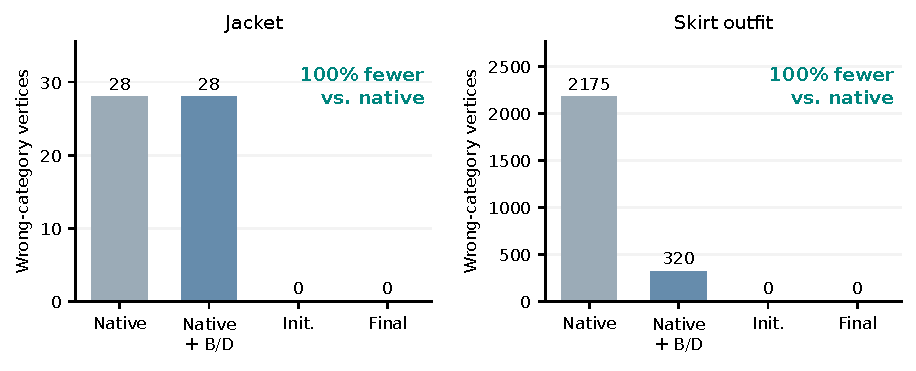
\includegraphics[width=\textwidth]{figures/semantic.pdf}
\caption{Semantic protection is already present before optimization. Wrong-category vertices decrease from 28 to 0 on the jacket and from 2,175 to 0 on the skirt outfit. Preserving the total body/dynamic split alone leaves 28 and 320 such vertices. ``100\% fewer'' refers specifically to this thresholded count in these two cases, not to overall accuracy or collision freedom.}
\label{fig:semantic}
\end{figure*}

\begin{table*}[t]
\centering\small
\caption{Allocation errors over all 8,885 jacket and 5,864 skirt-outfit vertices. $e_b$ and $e_d$ are absolute weight fractions. Pure-D pollution counts originally pure-dynamic vertices receiving body influence. Zero dynamic error in I and F is from this same-input audit; other writeback runs can have small storage residuals.}
\label{tab:semantic}
\begin{tabular}{llrrrr}\toprule
Case & Method & $N_{\mathrm{wrong}}$ & $e_b$ & $e_d$ & Pure-D pollution\\\midrule
\SemanticRows
\bottomrule\end{tabular}
\end{table*}

Table~\ref{tab:semantic} and Figure~\ref{fig:semantic} show the clearest benefit of the constraint system. Initialization eliminates every measured wrong-category vertex in both cases and preserves category shares within $5.03\times10^{-8}$. Final optimization maintains these properties. In the skirt outfit, native transfer assigns body weights to 1,855 originally pure-dynamic vertices. N+BD prevents this pollution but still produces 320 wrong-category vertices, demonstrating that a correct body/dynamic total does not determine correct anatomical ownership.

The zero-count result is consistent with the nonnegativity argument in Section~\ref{sec:formulation}. It verifies that classification, transfer, and writeback implement the constraint to the reported tolerance. It does not independently validate whether the original semantic labels represent the artist's intention in every possible asset.

\subsection{Response fitting and terminal refinement}
Table~\ref{tab:response} gives absolute errors, and Figure~\ref{fig:response} normalizes native error to 100 separately within each suite. Initialization improves macro response by 3.01\% on the jacket and 12.48\% on the skirt outfit relative to N. Final reductions are 5.539\% and 12.736\%, respectively. The stronger N+BD baseline reduces the skirt macro error before category constraints, but remains above the initialized and final results.

The largest improvement occurs on the jacket's 1,514-vertex terminal scope: final RMS decreases from 0.004943749 to 0.002435535, a 50.735\% reduction from native transfer. Relative to the historical macro output entering terminal refinement, the stage reduces error by 47.237\%. These percentages have different baselines and should not be interchanged.

\begin{figure*}[t]
\centering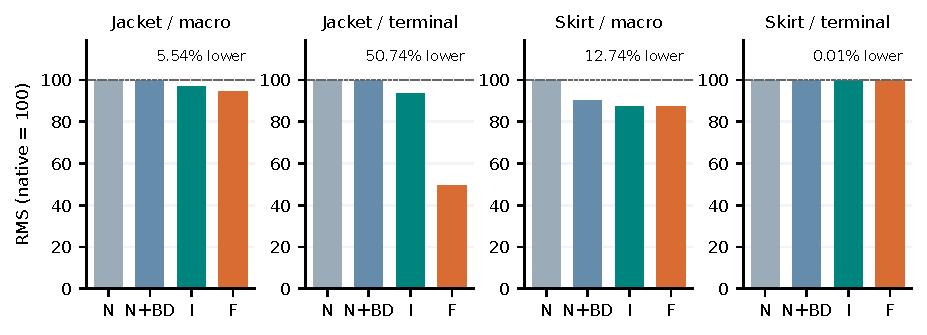
\includegraphics[width=\textwidth]{figures/response.pdf}
\caption{Held-out response normalized separately per suite. N: native; N+BD: native with body/dynamic allocation; I: initialization; F: final. The large jacket terminal improvement and small skirt terminal change are both retained. Similar RMS does not imply equivalent semantic allocation; compare Figure~\ref{fig:semantic}.}
\label{fig:response}
\end{figure*}

The skirt terminal scope is already close to its transferred reference under this metric. Its initialized RMS is marginally higher than native (a difference of approximately $3.08\times10^{-10}$), and final error decreases by only 0.012\% relative to native. We interpret this as a small local adjustment, not a substantial terminal improvement. Semantic preservation remains valuable even where the tested motion response is insensitive to differences in allocation.

\subsection{Initial cross-rig applicability and contact review}
The MMD-style skirt-outfit study is a limited cross-rig applicability experiment. It exercises source semantics with deformation helpers, preserved clothing chains, six-category initialization, macro optimization, and terminal refinement. Its reference is the \emph{fitted} mesh with original source weights frozen before transfer; it therefore tests weight/rig adaptation and does not isolate the complete pre-fitting shape-transport problem.

Authored cap intersections were reviewed locally rather than treated as a reason to abandon the whole garment. The final audit records unchanged exterior weights, zero dynamic-weight change, unchanged geometry, and no newly flagged contact vertices outside the reviewed cap mask. This demonstrates the practical value of scoped validation: local model limitations remain visible while changes elsewhere can be audited independently.

The contact result is an exception-reviewed outcome, not a strict global pass. The recorded strict contact gate did not pass, and six existing non-exempt selected vertices remained flagged. Thus this case supports contact non-regression by vertex-set membership in the recorded scope, while systematic collision robustness remains to be evaluated. No claim is made that unchanged contact membership bounds depth or guarantees every non-exempt vertex is collision-free. A full study would vary poses, garment layers, contact tolerances, and independently reviewed masks.

\subsection{Complex flat shoes}
The shoe pair contains 24,082 vertices. There are 153 extended-query vertices per side beyond the sampled foot's forward extent. Field repair decreases the recorded mean squared neighboring-proportion difference by approximately 45.3\% per side. This is a continuity statistic, not a direct perceptual or motion-error measurement.

\begin{table}[t]
\centering\small
\caption{Flat-shoe spatial branch, seven standard training poses and four held-out poses. Separation RMS is in scene units. Contact diagnostics refer to the recorded in-scope samples and triangle tests.}
\label{tab:shoe}
\begin{tabular}{lr}\toprule
Measurement & Value\\\midrule
Vertices (pair) & 24,082\\
Extended queries (each side) & 153\\
Held-out separation RMS, A & 0.0006319864\\
Held-out separation RMS, B & 0.0006004512\\
Relative reduction A$\to$B & 4.990\%\\
Max. body-share writeback error & $4.47\times10^{-8}$\\
Max. dynamic-weight writeback error & $2.98\times10^{-8}$\\
Detected in-scope triangle crossings & 0\\
Detected in-scope penetrating samples & 0\\
Maximum geometry change & 0\\\bottomrule
\end{tabular}
\end{table}

Optional separation fitting reduces held-out RMS by 4.990\% (Table~\ref{tab:shoe}). All four recorded validation poses have zero detected in-scope triangle crossings, ambiguous coplanar pairs, and penetrating samples. No unsupported body bone or unobserved knee influence appears in the writeback audit. This result supports the spatial branch on the tested shoes; it does not establish high-heel performance or continuous-time contact safety.

\subsection{Replay integrity and reproducibility}
The same-input baselines were generated in separate background Blender processes without changing production scenes. Shared target matrices replay exactly. Maximum body-pose replay discrepancy is below $6\times10^{-7}$ scene units; numerical native LBS agrees with Blender within $4\times10^{-7}$. Reference digests were checked, and archived initialization macro RMS and final terminal RMS were reproduced within $10^{-8}$.

The repository publishes numerical extracts, baseline definitions, scope sizes, pose identifiers, and local measurement hashes~\cite{artifact}. Figure and table generation reads these extracts directly. Private third-party meshes and complete scene archives are not redistributed, so the public artifact reproduces the reported presentation and arithmetic, not an independently runnable asset benchmark. Measurements describe archived runs; they are not fresh benchmarks of every subsequent UI or preset change. Runtime scaling, parameter sensitivity, and cross-method comparisons are left for a broader evaluation.

\section{Discussion and Limitations}
\paragraph{Why budgets are useful.}
Budget conservation turns an ambiguous nearest-surface choice into a restricted allocation problem. It is particularly effective when the source clearly excludes a category, as with a torso-only collar close to an arm. It also preserves mixed body/dynamic attachments that would be erased by deleting all body weights in dynamic regions. The method preserves source intent only to the extent that the source weights and reviewed roles encode that intent correctly.

\paragraph{Generalizing beyond one rig.}
The equations require category membership, correspondence of macro actions, and body-supported target candidates, not matching bone names or body topology. Additional target spine or twist segments enlarge the within-category distribution that can be fitted. They can also introduce correlated responses and ambiguity. A good semantic mapping and informative pose set remain necessary; more bones alone do not guarantee a better fit.

\paragraph{Limits of the reference.}
Paired garment vertices are required for motion transport. Remeshing without correspondence, strongly folded static fits, and unresolved helper semantics can invalidate local Jacobians or anatomical anchors. A stable-plus-gradient body component can require more structure than one category budget. The current protected-component interface is reserved rather than implemented. Future work can preserve selected subcomponents while fitting only the residual distribution.

\paragraph{Contact robustness as a scoped property.}
Explicit exception masks are useful for garments with known authored intersections and unadjustable fixed regions. They allow useful optimization and targeted validation to continue while keeping those limitations inspectable. Robust handling of such inputs should be distinguished from proving collision freedom. A claim of a strict pass must identify its pose set, sample set, mask, and tolerances. Neither the contact linearization nor an exception-reviewed historical case certifies all unsampled poses, self-collisions, other clothing layers, or body-shape edits.

\paragraph{Optimization scope and identifiability.}
The method fits body weights under fixed transforms; it does not recover physical dynamics. Pure-dynamic regions are intentionally outside body fitting. Strong conservation can leave too few degrees of freedom to satisfy a contact inequality. The regularized QP can choose a unique solution even when data alone are insufficient, so uniqueness does not establish physical correctness. The present implementation also does not promise a maximum number of influences per vertex. Later pruning or export constraints require revalidation.

\paragraph{Evaluation coverage.}
The reported evidence includes two garment conventions and one shoe pair. The initial cross-rig study supports feasibility, while a larger asset collection is needed to characterize generalization. Random auxiliary poses are implemented as a sampling extension, but their benefit awaits a dedicated ablation. Further experiments should isolate confidence fallback, semantic mappings, local transport, graph regularization, and terminal sampling, and report both motion and contact outcomes with complete configurations.

\section{Conclusion}
SBCST preserves per-vertex semantic influence allocation while adapting its within-category distribution to a new character. Native surface transfer remains useful, but is constrained by source ownership, fixed clothing dynamics, admitted body support, and reviewed finger policies. Proportion-aware motion fitting, local terminal refinement, and an alternative footwear separation objective share this contract. Local studies show exact exclusion of measured wrong-category influence within writeback tolerance and task-dependent improvements in held-out response. Explicit contact scopes allow authored limitations to be handled locally and transparently. The framework provides a practical basis for broader garment-retargeting evaluation without conflating semantic conservation, motion similarity, and collision guarantees.

% Start the final artifact/disclosure column after the conclusion.
\newpage
\paragraph{Availability and disclosure.}
Code, LaTeX source, measurement summaries, and build instructions are available in the project repository~\cite{artifact}. This is an independent technical manuscript, not a peer-reviewed publication. Implementation and manuscript preparation used AI-assisted development with human direction and review. Third-party assets retain their own rights and are not included in the paper artifact. The accompanying software is licensed under AGPL-3.0-only; see the repository for scope and notices.

\begin{thebibliography}{9}
\bibitem{ssdr} Binh Huy Le and Zhigang Deng. 2012. Smooth Skinning Decomposition with Rigid Bones. \emph{ACM Transactions on Graphics} 31, 6, Article 199. \href{https://doi.org/10.1145/2366145.2366218}{doi:10.1145/2366145.2366218}.
\bibitem{bbw} Alec Jacobson, Ilya Baran, Jovan Popovi\'{c}, and Olga Sorkine. 2011. Bounded Biharmonic Weights for Real-Time Deformation. \emph{ACM Transactions on Graphics} 30, 4. \url{https://igl.ethz.ch/projects/bbw/}.
\bibitem{blender} Blender Foundation. Data Transfer Modifier. \emph{Blender Manual}. \url{https://docs.blender.org/manual/en/latest/modeling/modifiers/modify/data_transfer.html}. Accessed September 2026.
\bibitem{osqp} OSQP Developers. The Solver. \emph{OSQP Documentation}. \url{https://osqp.org/docs/solver/index.html}. Accessed September 2026.
\bibitem{artifact} tomTomIEE. 2026. KK Modder BatchTool: SBCST implementation and measurement artifacts. \url{https://github.com/tomTom1010-IEE/KK_Modder-BatchTool}. Measurement snapshot: September 21, 2026.
\end{thebibliography}
\end{document}
